% !TEX root = ../../main.tex

\subsection{Impact of framework structure on transition mechanics}%
\label{dut:comparison}

While the discovery of the NGA transition in DUT-49 was a result 
of serendipity, it opens the door to a rational design approach 
to modify the extent and the location of the phenomenon. In principle,
there are several avenues that could be taken in order to tune the 
contraction mechanics.
\begin{itemize}
    \item Changing the range of metastability of the open pore state.
    \item Decreasing the porosity of the closed pore state.
    \item Increasing the capacity of the open pore form.
\end{itemize}
These factors are bound to be tightly interlinked, with a slight 
alteration in one possibly leading a shift in all. For example, the 
addition of a stabilizing group which would increase the tensile 
strength of the linker is also likely to decrease the porosity 
of the entire system.

There are a range of physicochemical modifications available to 
tune the properties of the framework, many already employed in the
MIL-53 and MIL-47 family of flexible MOFs.
Through functionalisation or modification of the linker, the strength of the guest-guest
and guest-host interactions is affected, as evidenced by the different
gate opening behaviour with nitrogen and water on several functionalised
versions on MIL-53~\cite{biswasNewFunctionalizedFlexible2011}.
In the case of DUT-49, moieties grafted to the central strut or changes
in the linker backbone are also likely to affect its buckling behaviour.
The use of a different metal as the node, has succeeded in changing the 
mechanical response of MIL-53~\cite{yotImpactMetalCentre2016}. This 
approach is likely have less impact on DUT-49, as the mechanism of 
contraction is due to linker flexibility.
A common rational design methodology is the so-called isoreticular design,
where topologically isomorphic MOFs are synthesised through progressive elongation
of the linker. Another path to controlling flexibility is manipulation of crystal 
size, as it has already been shown by \citet{krauseEffectCrystalliteSize2018}.
Finally, structural defects, of which a description was given 
in \autoref{def}, are another degree of freedom to consider for NGA 
tunability. Approaches such as mixed linkers synthesis and vacancy defects
may allow for fine-grain influence of framework stiffness.

\subsubsection{Behaviour of isoreticular materials}

The series of materials DUT-48, DUT-46, DUT-49, DUT-50 and DUT-151/DUT-152
was synthesised with the aim of studying the effect of linker 
elongation on the NGA step. It was found that the tetra-phenyl chain
in DUT-151 increased the pore size to the threshold 
where a secondary can form in the intracrystal voids, resulting 
in two identical interpenetrated nets. An attempt to introduce 
a bulky side-functionalisation in DUT-152 resulted in a similarly
interpenetrated material. \autoref{dut:fgr:dut-reticular} shows the
butane adsorption dataset recorded on the non-interpenetrated versions.

\begin{figure}[htb]
    \centering
    \begin{subfigure}{0.33\linewidth}
        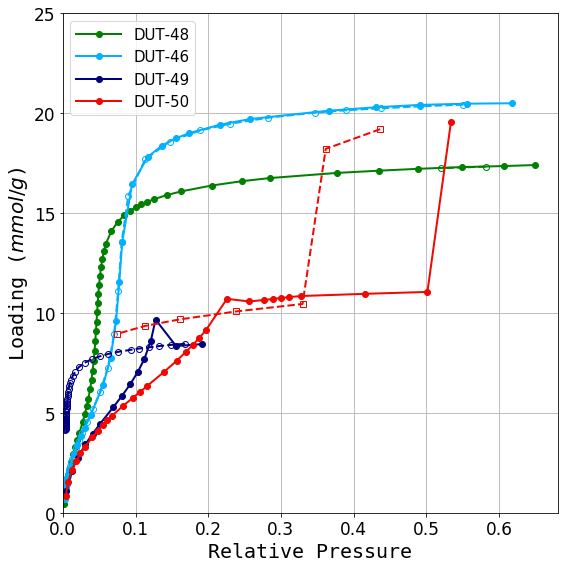
\includegraphics[width=\linewidth]{butane/dut-reticular-reg}%
        \caption{}\label{dut:fgr:dut-reticular-reg}
    \end{subfigure}%
    \begin{subfigure}{0.33\linewidth}
        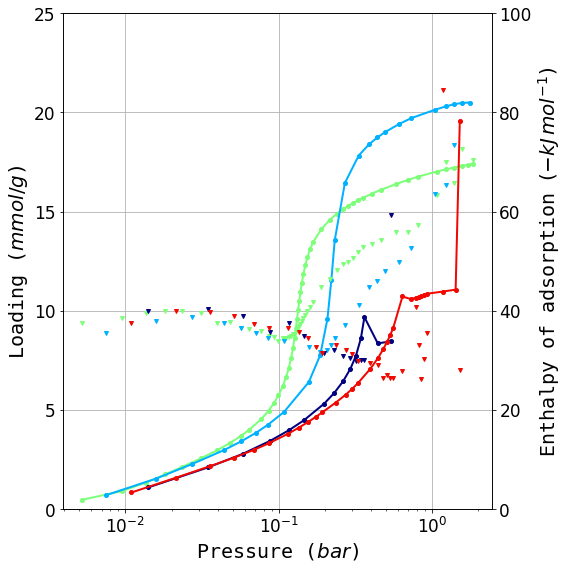
\includegraphics[width=\linewidth]{butane/dut-reticular-log}%
        \caption{}\label{dut:fgr:dut-reticular-log}
    \end{subfigure}%
    \begin{subfigure}{0.33\linewidth}
        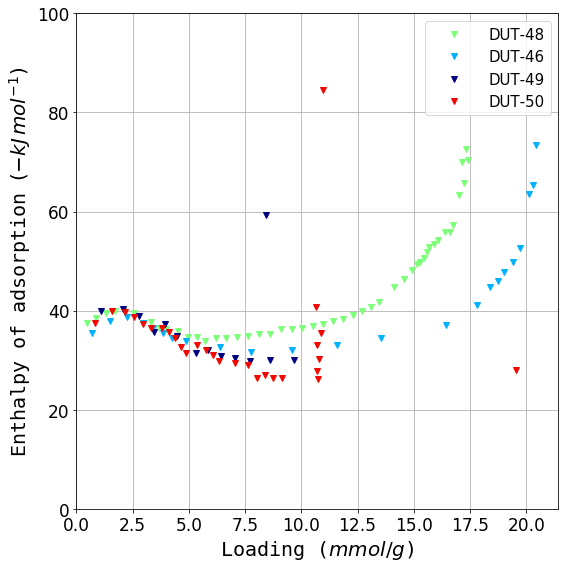
\includegraphics[width=\linewidth]{butane/dut-reticular-enth}%
        \caption{}\label{dut:fgr:dut-reticular-enth}
    \end{subfigure}%
    \caption{(a) Experimental adsorption isotherms for DUT-48, DUT-46, DUT-49 and 
    DUT-50. Enthalpy points are omitted for clarity. (b) A logarithmic plot of 
    isotherms and enthalpy curves, to highlight the low pressure region. 
    (c) Enthalpy as a function of loading.}%
    \label{dut:fgr:dut-reticular}
\end{figure}


Indeed, the results follow a predictable trend. First, it is worth 
noting that, as seen in \autoref{dut:fgr:dut-reticular-reg}, only DUT-49 
and DUT-50 undergo an \textbf{op/cp} transition. This confirms that 
a shorter linker imparts the resulting MOF with a more stable backbone,
raising the strain required in order to collapse the framework.
The desorption branch of the non-flexible materials completely 
overlaps the adsorption branch in both isotherm and enthalpy, further
confirming the small error in measurement (available in 
\autoref{appx:dut:fgr:dut-46-adsdes}).
With an increase of linker size, a larger pore volume and consequently
a higher amount of butane can be adsorbed in the open pore form. 
The increase in pore size is also responsible for a shift in the pressure 
of condensation, or pore filling step.

In DUT-50, the structure is seen to re-open around \(0.5~p/p_0\), although 
the pressure is not high enough to completely transition to the
\textbf{op} form. The collapse to the closed phase in the desorption
branch achieves a lower plateau than in the adsorption branch,
suggesting an incomplete \textbf{op/cp} transition as seen in one 
of the isotherms on DUT-49 in the previous section.

One surprising finding is that the enthalpy curves 
(\autoref{dut:fgr:dut-reticular-enth}) present a near
identical behaviour and differential enthalpy of adsorption in the 
low pressure region, characterized by a slight increase up to 
\SI{40}{\kilo\joule\per\mol} followed by a drop-off. The adsorption
mechanism and surface characteristics are therefore \textit{common} to 
all four materials. The shift of the enthalpies of adsorption to lower 
values at higher loadings from DUT-46 to 50 is expected, with the increase
in pore size leading to a progressive decrease of the contribution 
of dispersion interactions with the guest, which could also be 
referred to as a confinement effect. The the steep uptake in the isotherm
is indicative of a cooperative adsorption mechanism similar to a fluid
condensation, accompanied by an increase in the contribution of 
guest-guest interactions to \(\Delta_{ads} \dot{h}\).

As neither DUT-48 and DUT-46 show any phase transition with
butane at this temperature, the question arises whether their frameworks
can still undergo a structural contraction. A combined simulation and 
mechanical pressure study was performed on DUT-48 in parallel to the 
microcalorimetry experiments, which can be found in the paper 
published in collaboration with the TU Dresden, Chimie ParisTech and 
ICGM groups~\cite{krauseAdsorptionContractionMechanics2018}.
In brief, DFT optimisations of a single linker molecule under increasing
stress show that buckling of the molecule is still possible, albeit
at a much higher stress. Constant volume (N, V, T) molecular dynamics
simulations of the evolution of the system free energy with decreasing
unit cell volume have shown that, while a \textbf{cp} phase for DUT-48
exists, the increased tensile strength of the central backbone leads
to an increase in both the free energy of this state and the activation
energy required to enter it compared to DUT-49. To prove that structural
transition can still take place, mercury intrusion experiments are 
carried out on both DUT-48 and DUT-49. The intrusion/extrusion 
curves on both materials show that an \textbf{op/cp} transition takes
place, although with a much higher external pressure in the case 
of DUT-48 (\SI{65}{\mega\pascal} vs.\ \SI{35}{\mega\pascal}). A similar 
approach on all other materials in this series reveals a very clear
trend in both energy of the \textbf{cp} form and pressure required 
for the transition.

The interpenetrated materials DUT-151 and DUT-152 show a very different 
isotherm shape and enthalpy curve, as seen in 
\autoref{dut:fgr:dut-reticular-interp}.

\begin{figure}[htb]
    \centering
    \begin{subfigure}{0.5\linewidth}
        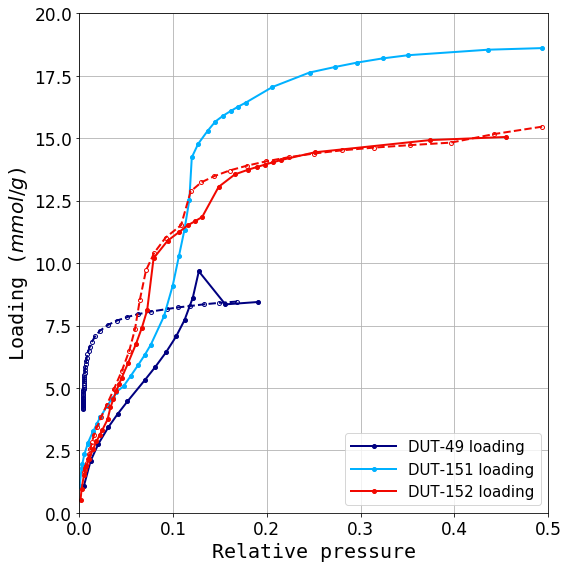
\includegraphics[width=\linewidth]{butane/dut-reticular-interp-reg}%
        \caption{}\label{dut:fgr:dut-reticular-interp-reg}
    \end{subfigure}%
    \begin{subfigure}{0.5\linewidth}
        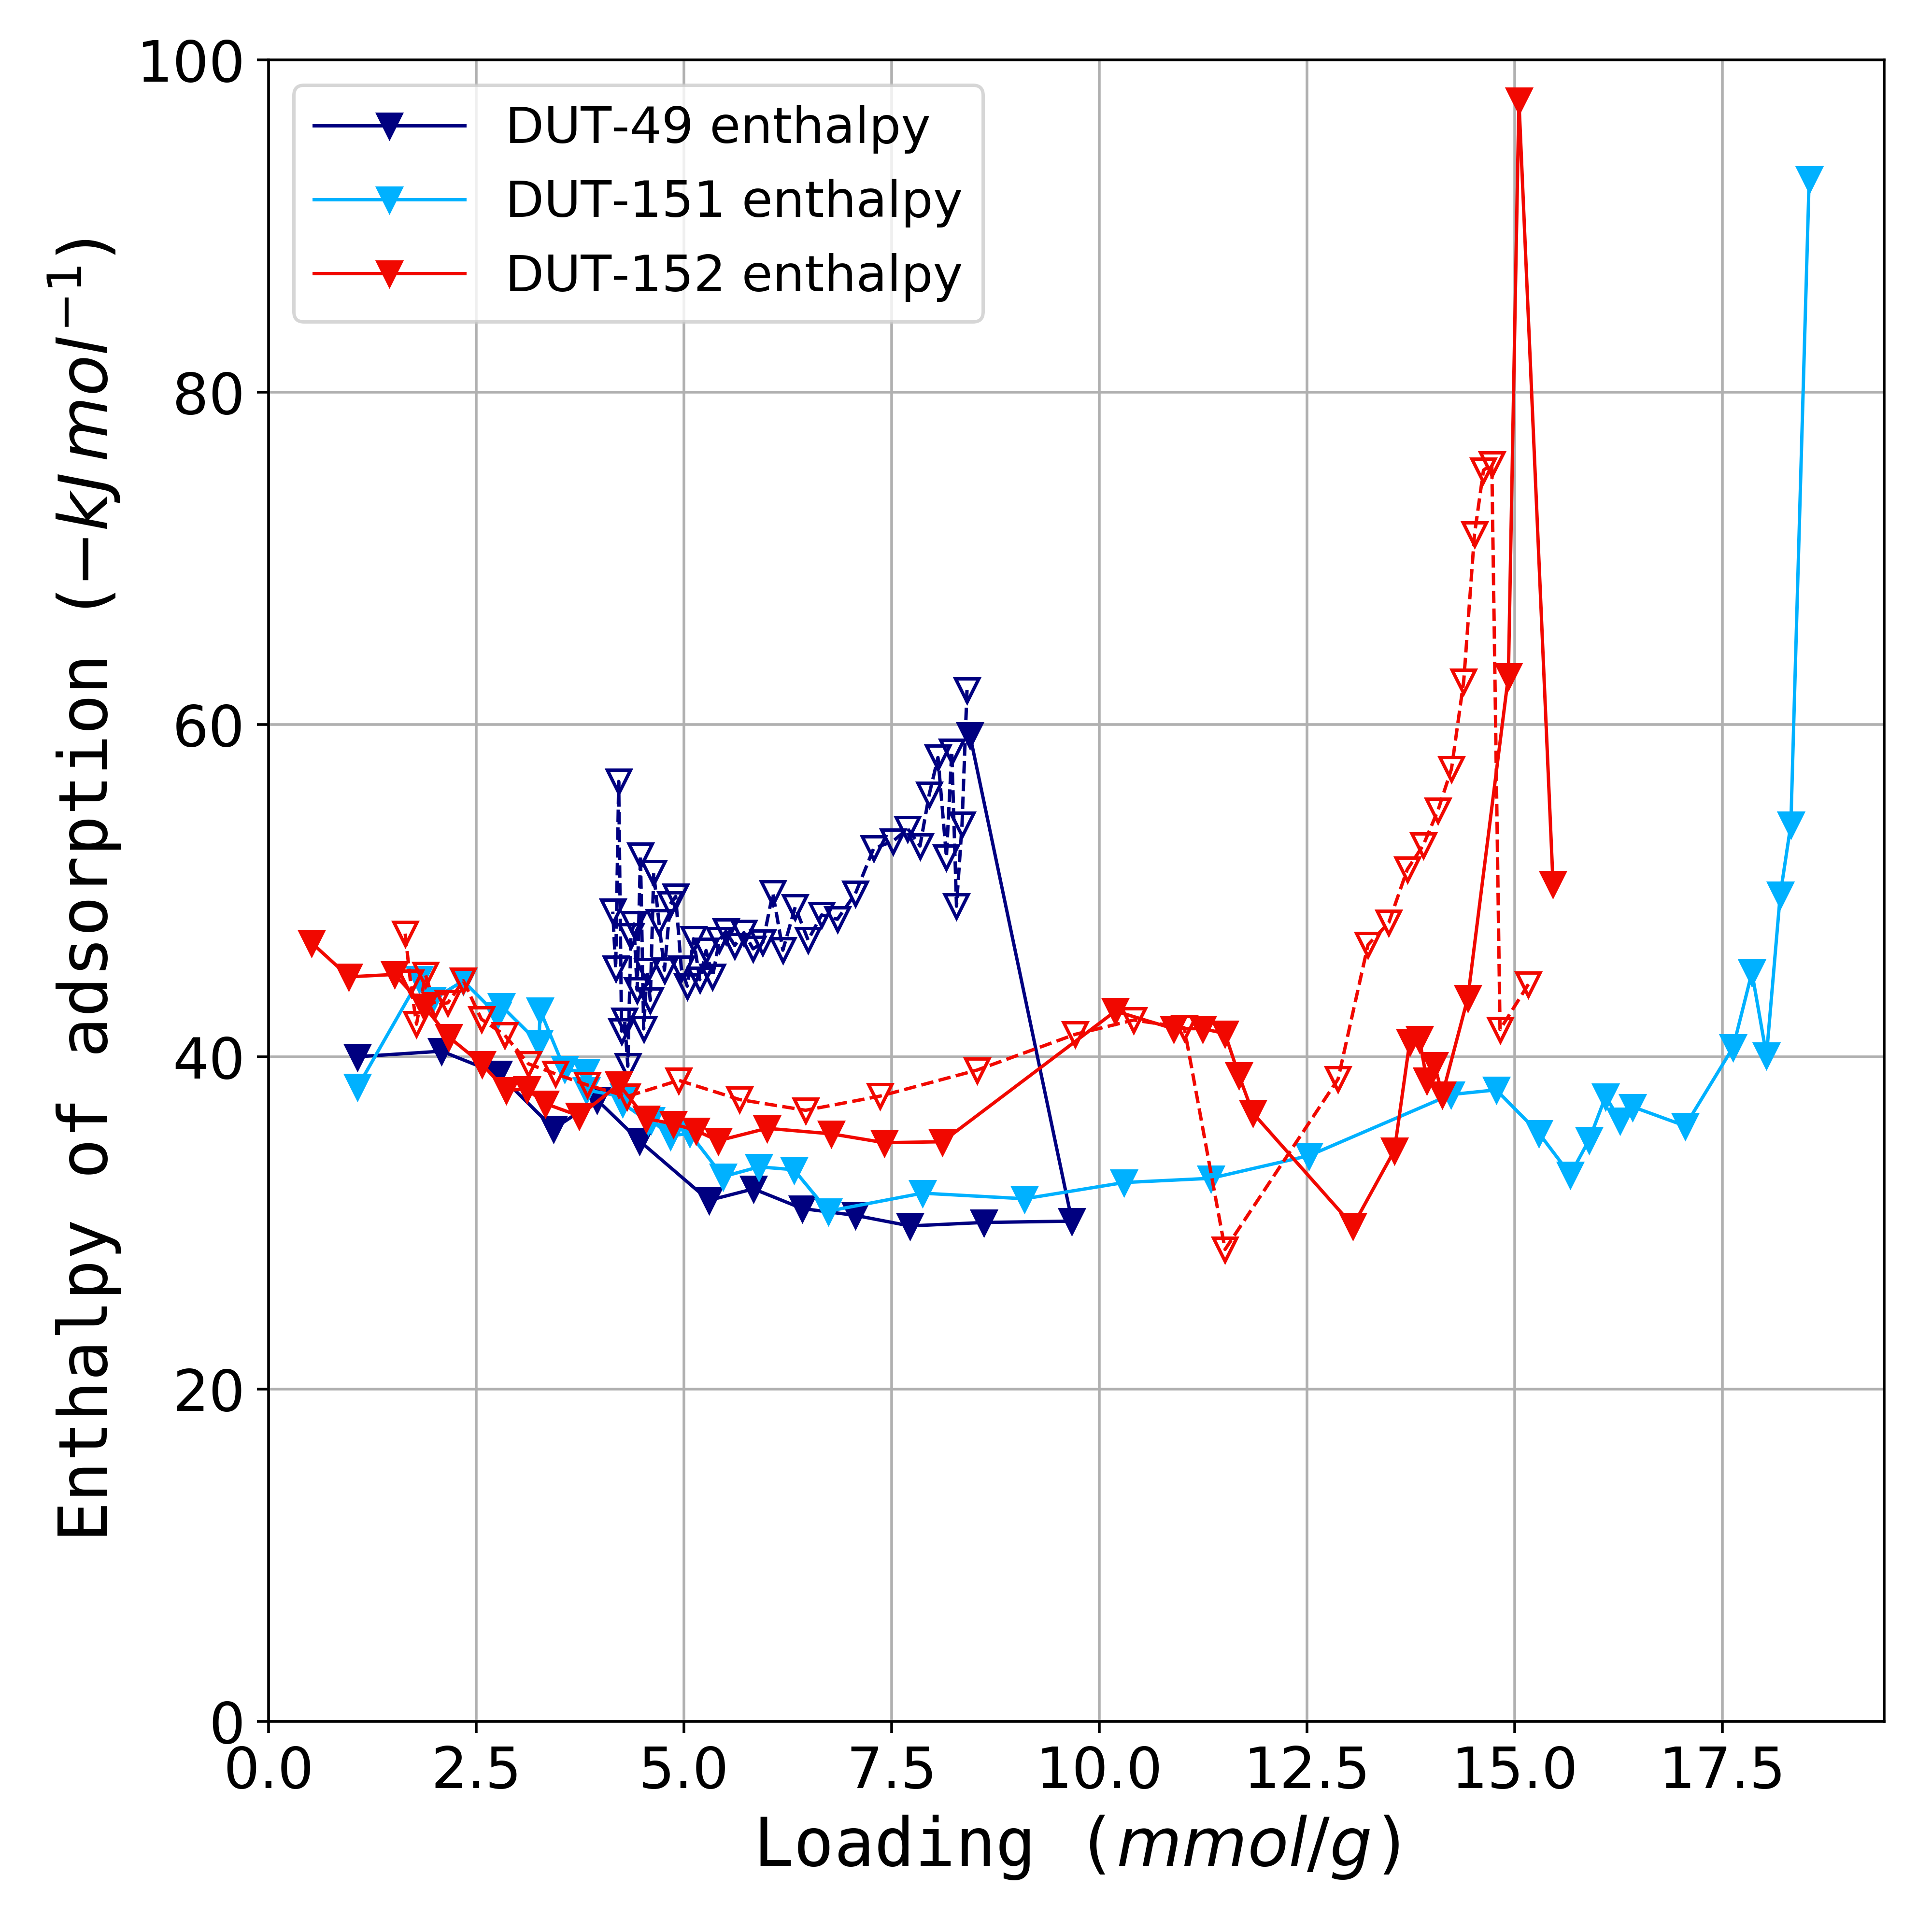
\includegraphics[width=\linewidth]{butane/dut-reticular-interp-enth}%
        \caption{}\label{dut:fgr:dut-reticular-interp-log}
    \end{subfigure}%
    \caption{The (a) isotherms and (b) enthalpy curves of the
    interpenetrated materials DUT-151 and DUT-152. Shaded regions
    are guides for the eye.}%
    \label{dut:fgr:dut-reticular-interp}
\end{figure}


\subsubsection{Behaviour of ``reinforced'' linker analogues}
